\subsection{MELD (NLT 40nm)}

\subsubsection*{Simple Definitions}

\begin{itemize}

  \item MELD: A \textbf{directive} proword for the flight to cease sanitization
    scanning and focus radar energy on the specific group targeted, then Sort

  \item SORT: A process or directive that assigns targeting within a single
    group to each aircraft in the flight

  \item AZ: Short for Azimuth (left right)

  \item EL: Short for Elevation (up and down)

  \item Bar: Single sweep of radar across an AZ at the same EL

  \item HOOK: RIO selects a radar contact on TID using the Hand Control Unit
    full action.

\end{itemize}


\subsubsection*{General}

The MELD takes place one 'time segment' before the shot, and is important for
these reasons:

\begin{itemize}
  \item It's a timeline directive call made prior to weapons employment -
    objective is to remain on timeline and not shoot late

  \item It serves to ensure the radar is scanning a good volume for precise
    updates in TWS

  \item It focuses the contract sort mechanics

  \item The WM RIO will hook the sorted target and report so that the flight
    Lead knows the flight is sorted prior to employment

\end{itemize}

\subsubsection*{Process}

\sidebyside{0.65}{%
  \begin{itemize}

    \item \href
      {http://www.heatblur.se/F-14Manual/weapons.html\#id4}
      {http://www.heatblur.se/F-14Manual/weapons.html}

    \item After the directive, RIOs will change radar mode TWS Manual, 20AZ, 4
      bar EL, 50nm scale and steer the AZ towards the centre mass of the group.

    \item Contract sort silent

    \begin{itemize}
      \item \textbf{FL}: Left, Lead, High
      \item \textbf{WM}: Right, Trail, Low
    \end{itemize}

    \item They will HOOK the contract sort on TID and select 'Next Launch' on
      the RIO armament Panel

  \end{itemize}
}{%
  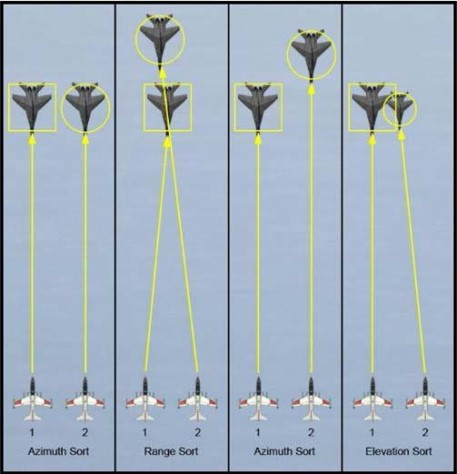
\includegraphics[width=\textwidth,align=t]{bvr/sort}
}

\subsubsection*{Unable to Sort Process}

If unable to accurately determine sort, there must be a process to quickly
decide what to do:

\begin{itemize}
  \item WM RIO will report on Flight channel, "Unable Sort"

  \item Lead RIO will respond with "Drop 'em" and employ on BOTH contacts from
    TWS

  \item WM RIO will continue to monitor for that Bandit in case of merge
\end{itemize}

\subsubsection*{Example}

\textbf{FL RIO (Pri):} "Spectre 1, MELD, BRAA, One-Zero for Forty, nineteen
thousand."\\
\textbf{WM RIO(Pri):} "2, Sorted"

\boxed{
  Flight Lead RIO calls the flight to direct radars at the bearing, range and
  altitude, expecting sort to be via contract. FL RIO hooks the left target and
  presses 'NEXT LAUNCH' on the RIO armament panel. WM RIO does same with right
  contact and calls that he is sorted.
}
